
\chapter{The Compact Muon Solenoid Experiment at The CERN Large Hadron Collider}
\label{chap:CmsExp}

\section{The \LHC}

The Large Hadron Collider (LHC) at CERN near Geneva is the world's newest and
most powerful tool for Particle Physics research. It is designed to collide proton beams with a
centre-of-mass energy of 14 TeV and an unprecedented luminosity of 10$^{34}$ cm$^{-2}$s$^{-1}$
. It can also collide heavy (Pb) ions with an energy of 2.8 TeV per nucleon and a peak luminosity of 10$^{27}$ cm$^{-2}$
s$^{-1}$


\begin{figure}
  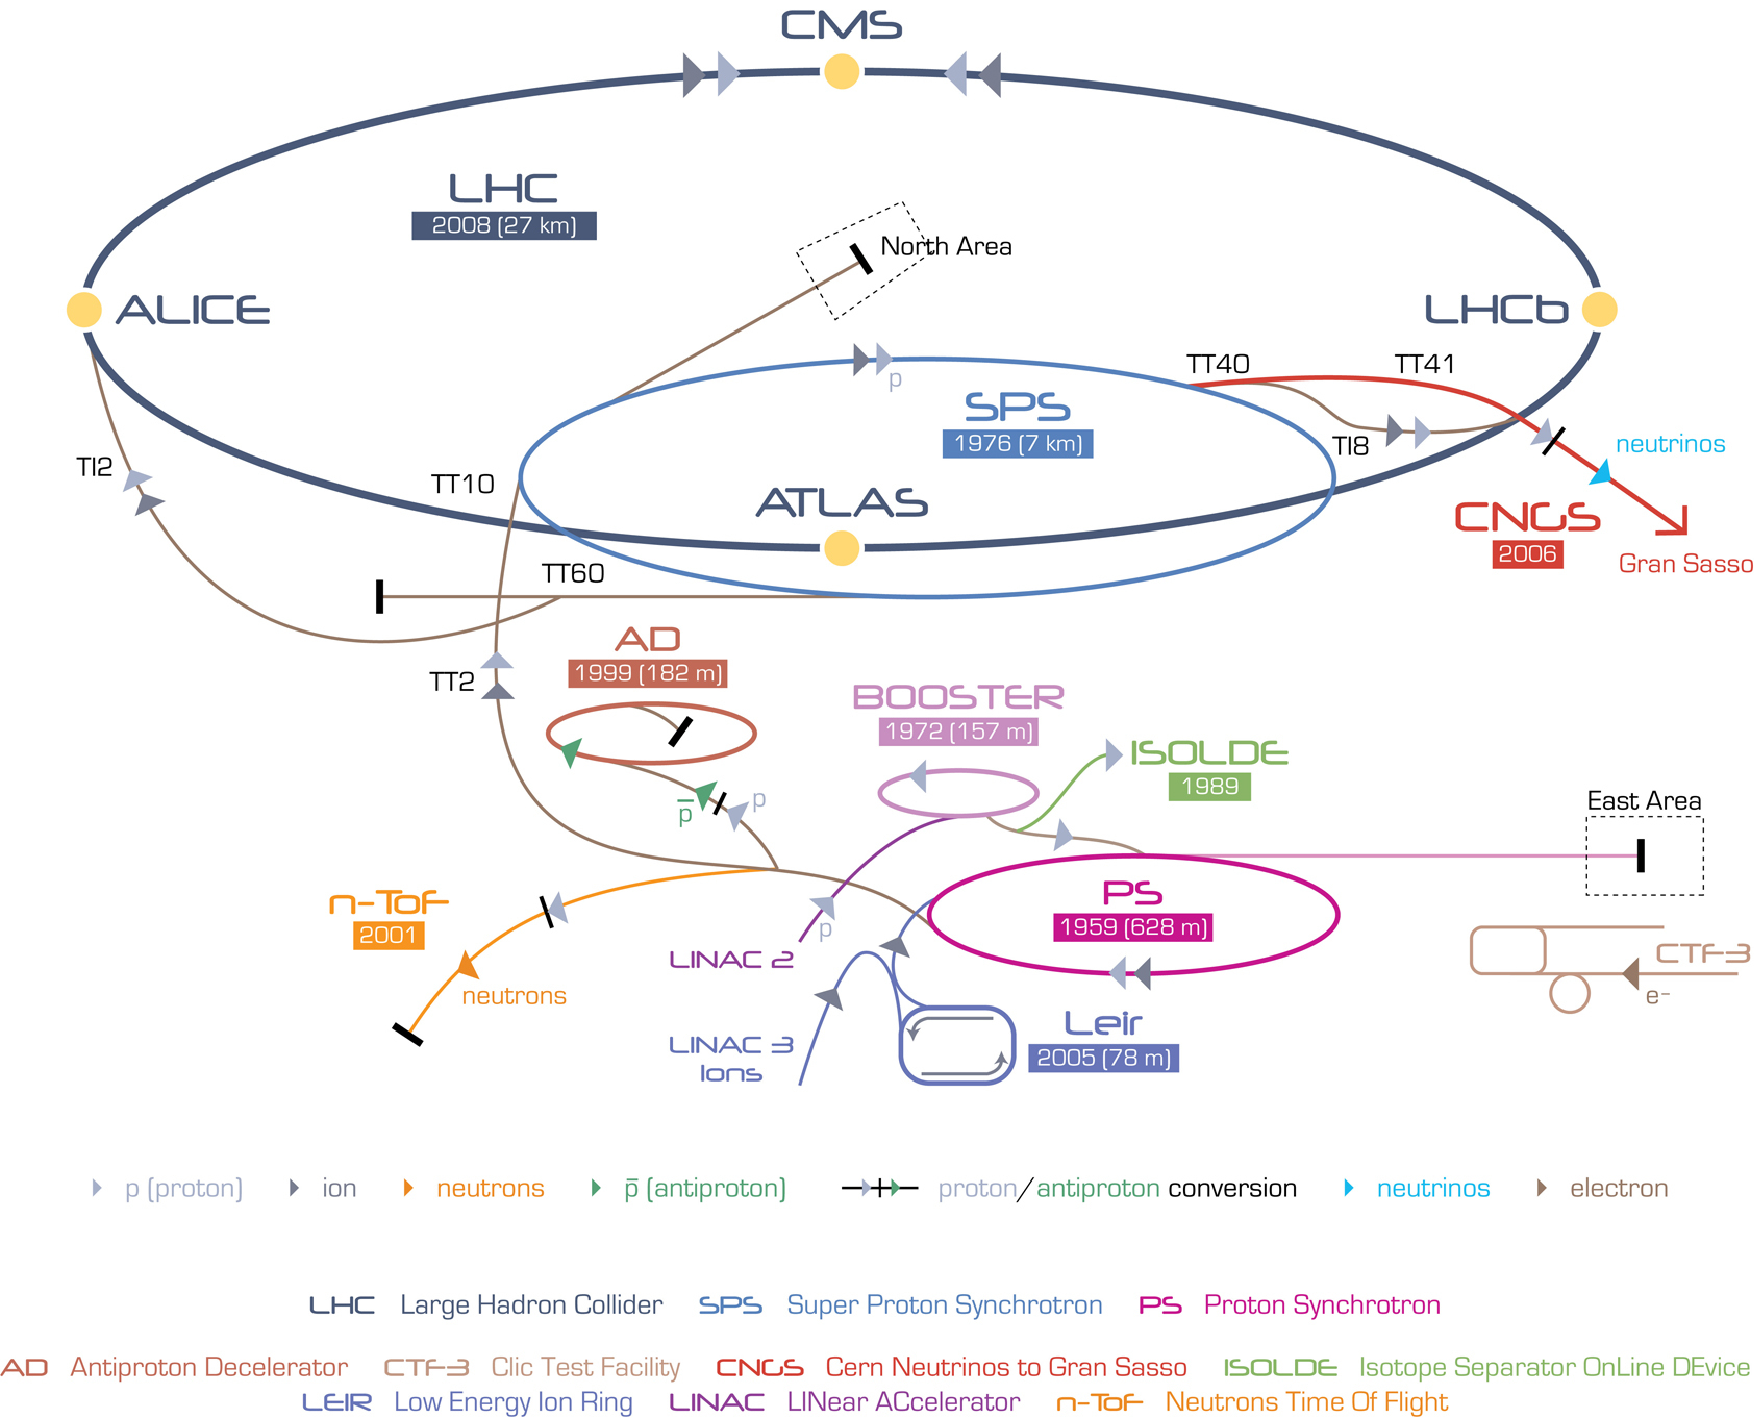
\includegraphics[width=\hugefigwidth]{chap_CMSDetector_figures/Cern-Accelerator-Complex}
  \caption[CERN accelerator complex]%
  {LHC  accelerator complex}
  \label{fig:CERNAccComplex}
\end{figure}




\begin{figure}
  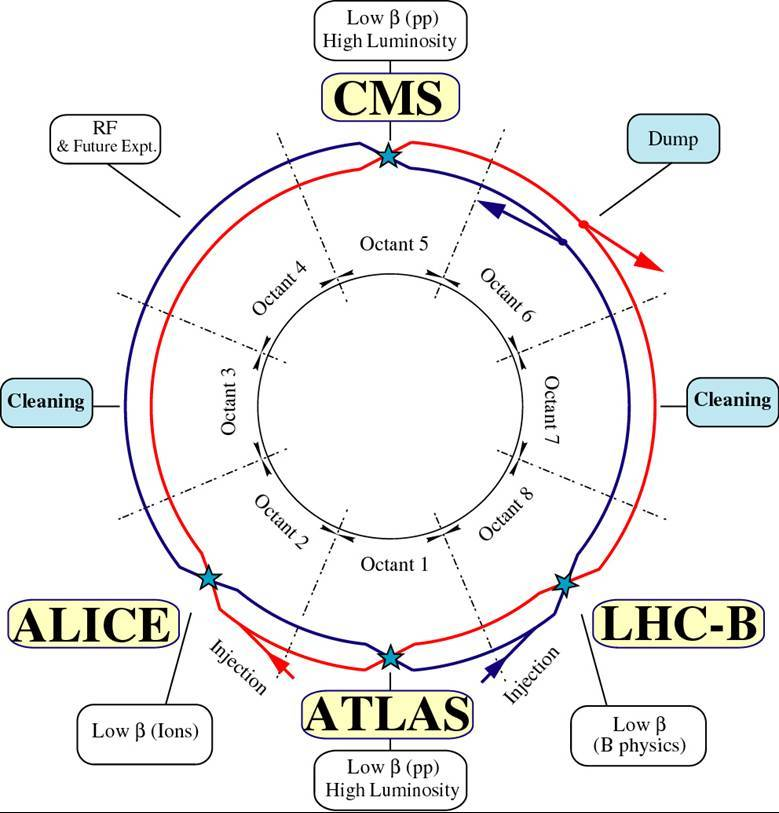
\includegraphics[width=\mediumfigwidth]{chap_CMSDetector_figures/lhc-schematic}
  \caption[LHC ring]%
  {LHC ring}
  \label{fig:LHCRing}
\end{figure}

It has circumference of 27 kms and is placed in a tunnel, 175 meters under the ground near Geneva.
The tunnel was originally built for the Large Electron-Positron collider \cite{LEP}. 
For the LHC operation, they have been upgraded to provide beams of protons for 
collisions at unprecedented energies. 
Technical limitations in the production and storage of antiprotons led to the de- 
cision to build a proton-proton collider. Accelerated electrons and positrons suffer 
large energy loss due to the synchrotron radiation, which is proportional to 
$\frac{E^4}{(Rm^4)}$, 
where E is the electron energy, m is the particle's mass and R the accelerator radius. 
Therefore, only massive charged particles could have been used, e.g. protons and 
heavy nuclei, in order to obtain energies of the order of TeV at the fixed accelerator 
radius. 

\subsection{The Accelerator Chain}

The LHC is constituted by 1232 super-conducting dipole magnets each 15 m long, 
delivering a 8.3 T magnetic field to let the beams circulate inside their trajectories 
along the 27 km circumference. Two vacuum pipes are utilized to let beams circulate 
in opposite directions. 
More than 8000 other magnets are utilized for the beam 
injection, their collimation, trajectory correction, crossing. All the magnets are kept 
cool by superfluid helium at 1.9 K temperature. The beams are accelerated from 
450 GeV (the injection energy from the SPS) to 7 TeV with 16 Radio Frequency 
cavities (8 per beam) which raise the beam energy by 16 MeV each round with an 
electric field of 5 MV/m oscillating at 400 MHz frequency. Before the injection into 
the LHC, the beams are produced and accelerated by different 26 components of the 
CERN accelerator complex. Being produced from ionized hydrogen atoms, protons 
are accelerated by the linear accelerator LINAC, Booster and the Proton Synchrotron 
(PS) up to 26 GeV energy, the bunches being separated by 25 ns each. The beams are 
then injected into the Super Proton Synchrotron (SPS) where they are accelerated 
up to 450 GeV. They are then finally transferred to the LHC and accelerated up to 
7 TeV energy per beam.


Figure \ref{fig:CERNAccComplex} shows the full CERN accelerator complex.


In addition to $p + p$ operation, the LHC had 
heavy nuclei $(Pb + Pb)$ collisions in 2009 and 2011 
 with an energy of 2.76 TeV per nucleon. The availability of high energy heavy-ion beams at energies
over 30 times higher than at the present other accelerators will allow us to
further extend the range of the heavy-ion physics program to include studies
of hot nuclear matter.


%\section{Lattice layout}
The two LHC symmetrical rings are divided into eight octants and arcs and
eight straight sections approximately 528 $m$ \ref{fig:LHCRing}. The two high luminosity
experimental insertions are located at diametrically opposite straight
sections: the A Toroidal LHC ApparatuS (ATLAS) experiment is located
at Point 1 and the Compact Muon Solenoid (CMS) experiment
at Point 5. The other two large experiments, A Large Ion Collider Experiment
(ALICE) and Large Hadron Collider beauty (LHCb), are located
at Point 2 and at Point 8, respectively, where the machine reaches a lower
luminosity of $L = 5 \, \times \,10^{32} cm^{-2}s^{-1}$. The remaining four straight sections do
not have beam crossings. The two beams are injected into the LHC in two
different octants, octant 2 and octant 8 respectively for clockwise and anticlockwise
beam. The octants 3 and 7, instead, contain two collimation systems
for the beam cleaning. 



\section{Luminosity}
The number of events per second generated in the LHC collisions is given by :
N = $L.\sigma$
where $\sigma$ is the cross section for the collisions process under study and $L$ the
machine luminosity. The machine luminosity depends only on the beam parameters and can be written, 
for a Gaussian beam distribution, as:

% thesisDongho ends

% PromptChic_CMS_2012.pdf 

\begin{equation}
\label{eq:Lumi}
L = \frac{n \cdot \,f_{rev}\cdot \,N_{1} \cdot \, N_{2}}{A^{eff}_T}
\end{equation}

where $A^{eff}_T$ is the effective transverse area of the proton beam, $n$ is the number of packets
the beam is splitted to and $f_{rev}$ is the frequency of revolution around the ring. $N_{1}$ and $N_{2}$ are
the number of protons in each packet. With respect to other high energy colliders, the design
luminosity of LHC is several magnitudes larger. This is needed because LHC is designed
to discover new particles at TeV scale. At these scales the interaction rates with momentum
transfers more than 1 TeV are very low. Therefore more data needs to be collected which can
only be achieved by having large luminosity.

% PromptChic_CMS_2012.pdf ends

% thesisDongho 
The LHC luminosity is not constant over physics a run, but decays due to the
degradation of intensities and emittance of circulating beams. The main cause
of the luminosity decay during normal LHC operation is the beam loss from
collisions.

\section{Compact Muon Solenoid}

The CMS experiment is a general purpose proton-proton detector designed to run 
at the highest luminosity of LHC. Figure \ref{fig:CMSFigure} gives a 3D structure view of the 
CMS detector.
The design of the CMS detector is based on a compact superconducting 
solenoid coupled with a muon detector system for optimized muon detection.
Superconducting solenoid provides a strong magnetic field of 3.8 $T$. 
Inside it, the inner tracking comprises a Pixel detector
surrounded by the Silicon Strip detector. Its high granularity (70
millions pixels, 10 millions strip) and precision ensures good track reconstruction
efficiency. It is surrounded by Electromagnetic calorimeter (ECAL) made
of 76000 lead tungstate crystals grouped in 36 barrel and 4 endcap supermodules.
The brass-scintillator sampling hadron calorimeter (HCAL) completes
the in-coil detectors. To ensure hermeticity the in-coil calorimetric system is
extended, away from the central dector, by the hadron outer detector (HO)
and a quartz fiber very forward calorimeter (HF) to cover $\eta le $< 5. Outside the
solenoid a muon system is built in the magnet steel return yoke. It's formed by
4 stations of muon chambers: Drift Tube (DT) in the barrel region, Cathode
Strip Chambers (CSC) in the endcap, Resistive Plate Chamber (RPC) in both
parts, providing muon detection redundancy. 







Two trigger levels are employed in CMS. The Level-1 Trigger (L1) is implemented using 
custom hardware processors and is designed to reduce the event rate to 100 kHz during LHC operation
using information from the calorimeters and the muon detectors. It operates nearly 
dead time-free and synchronously with the LHC bunch crossing
frequency of 40 MHz. The High Level Trigger (HLT) is implemented across a
large cluster of commodity computers referred to as the event filter farm, and
provides further rate reduction to $\mathcal{O}$(100) Hz using filtering software applied
to data from all detectors at full granularity. The overall dimension of CMS
are a length of 21.6 $m$, a diameter of 14.6 $m$ and a total weight of 12500 tons.


A slice of the transverse view of the CMS detector
is shown in Figure \ref{fig:CMSFigureSlice}. The principle of detection of charged and neutral particles in
the various sub-detectors is shown. All charged particles leave signals in the inner
tracking system. Electrons and photons deposit their energy in the electromagnetic
calorimeter. Charged Hadrons (K$^{\pm}$, $\pi^{\pm}$ ...) and neutrons deposit their energy in the
hadronic calorimeter. Muon is a particle which passes through calorimeters without
interacting much, but which leaves a track of its passage in the muon chambers.
Neutrinos, barely interacting, will escape from all direct detections. While adding
the transverse momenta of all the particles detected by the detector, one can determine
the imbalance of energy in the transverse plane, so called the missing transverse
energy.

\begin{figure}
  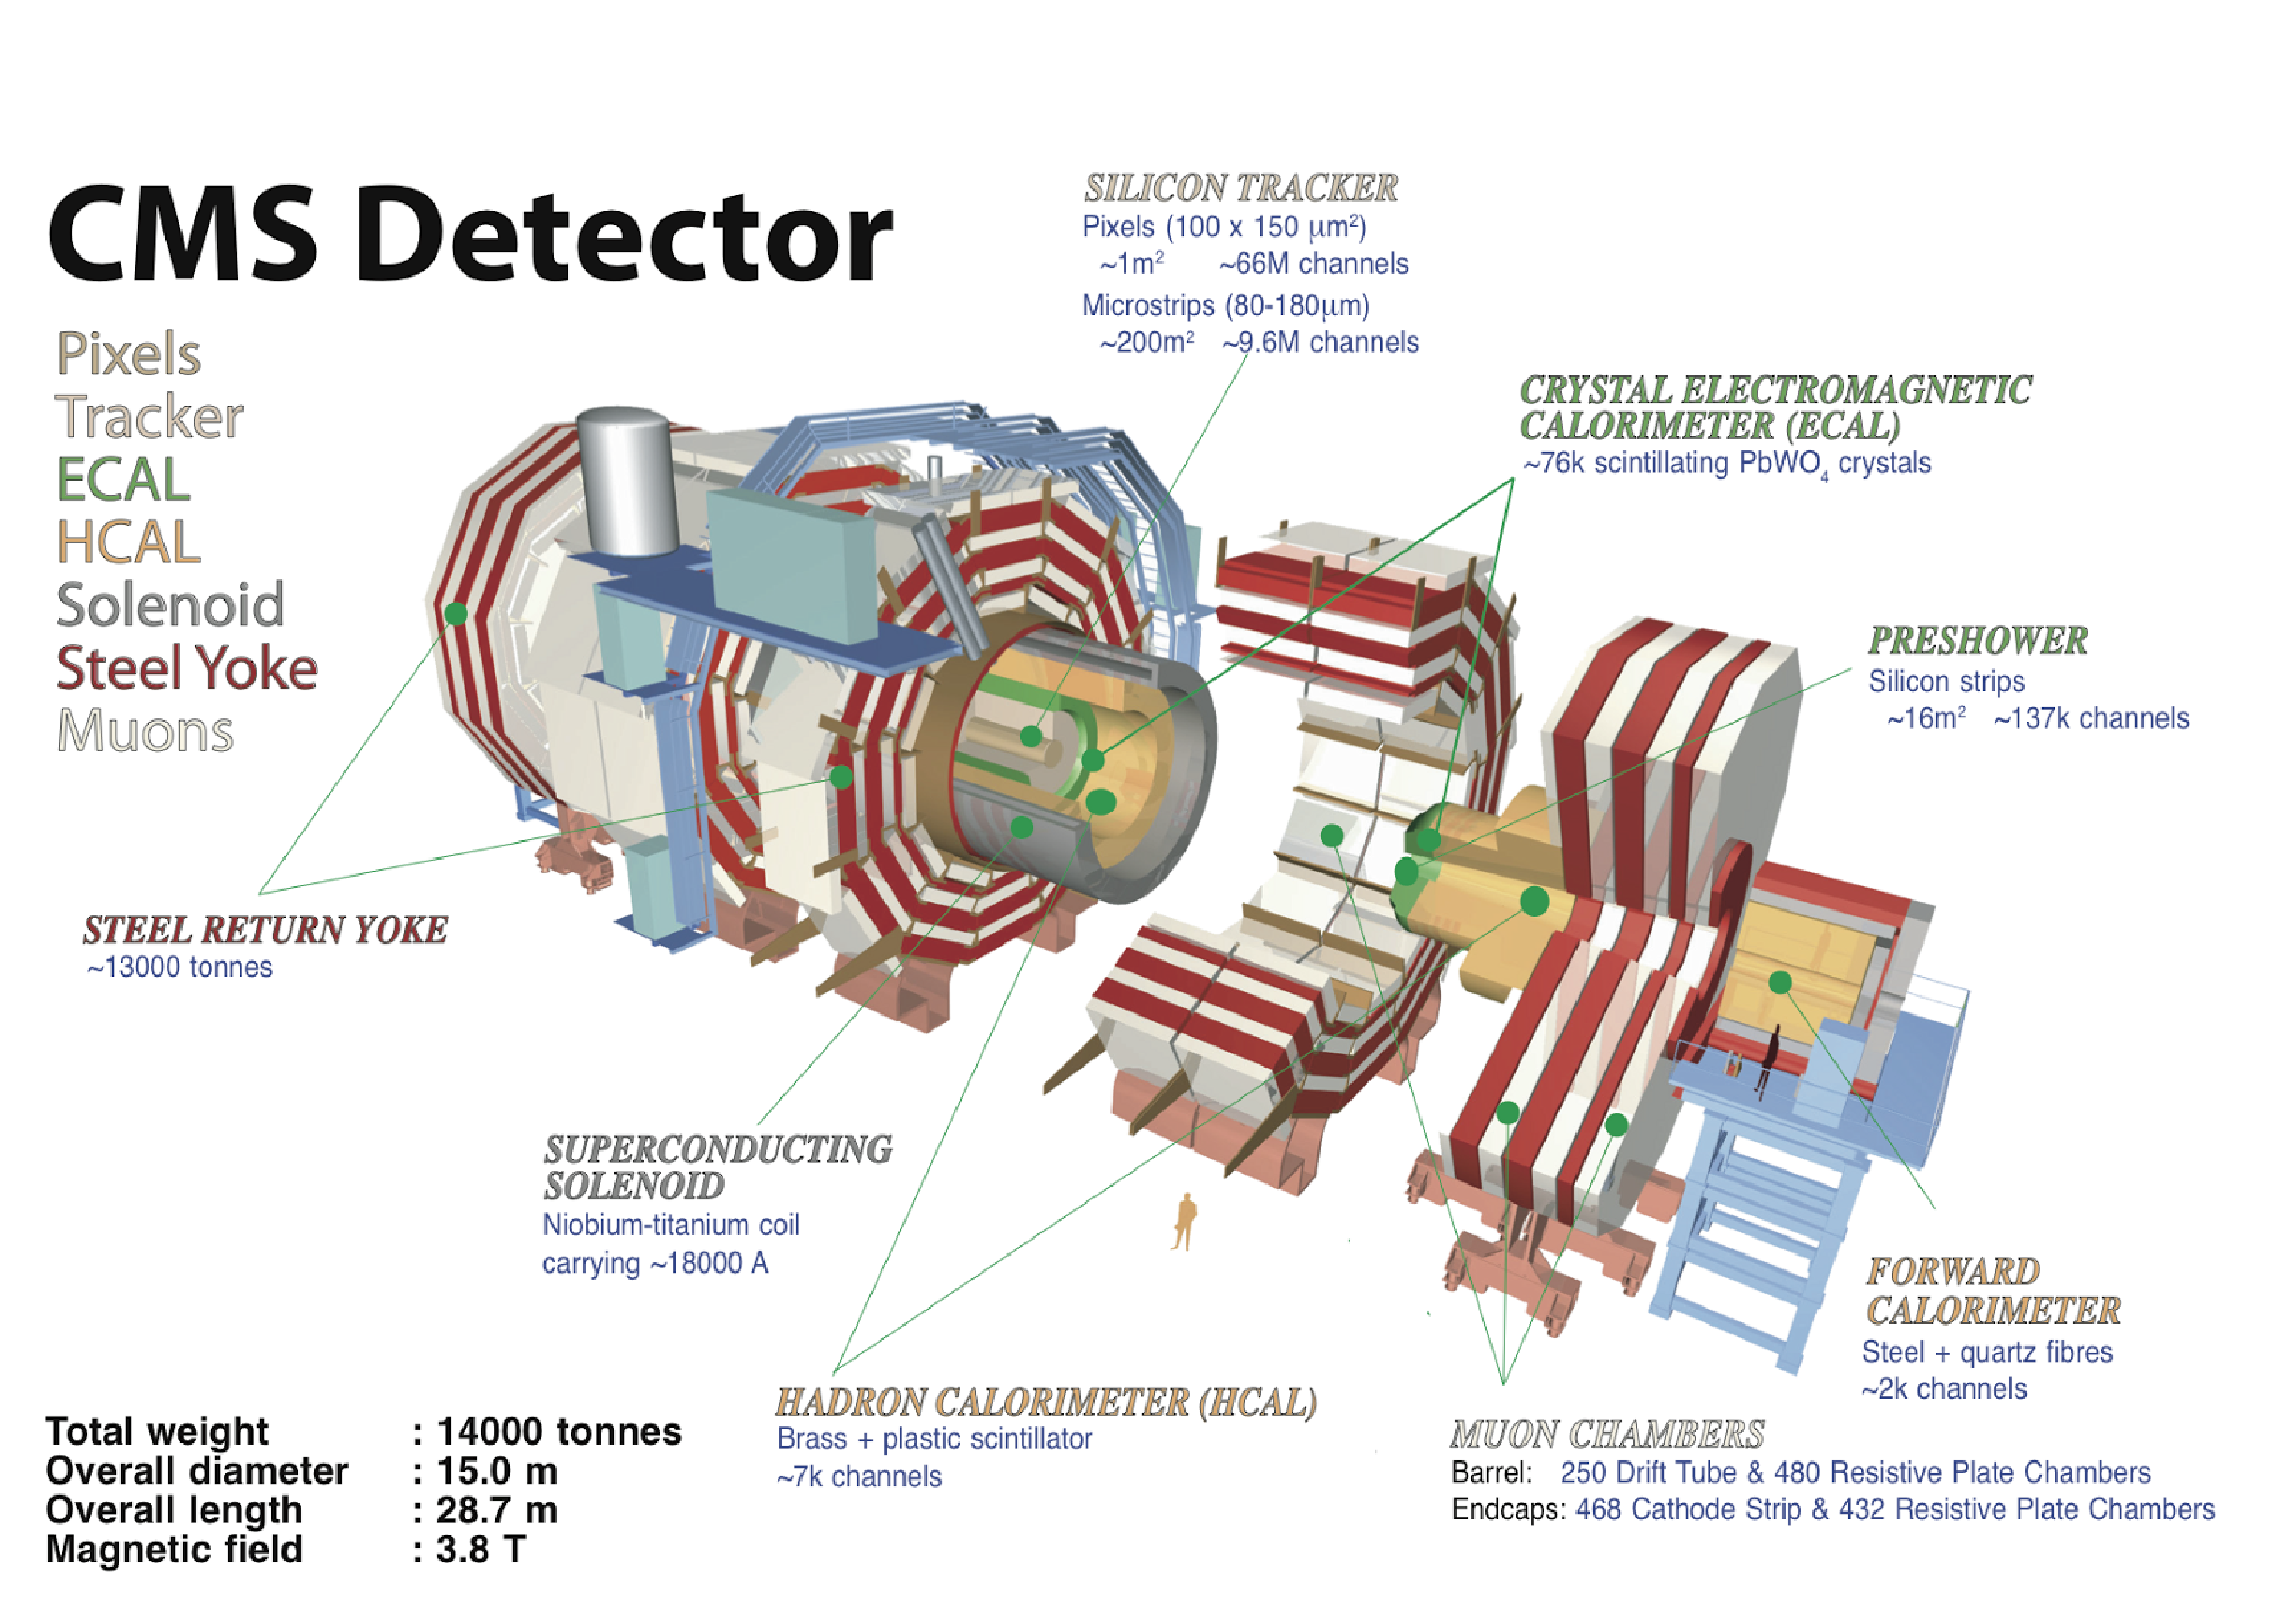
\includegraphics[width=\hugefigwidth]{chap_CMSDetector_figures/CMS}
  \caption[CMS Detector figure]%
  {CMS detector figure}
  \label{fig:CMSFigure}
\end{figure}



\begin{figure}
  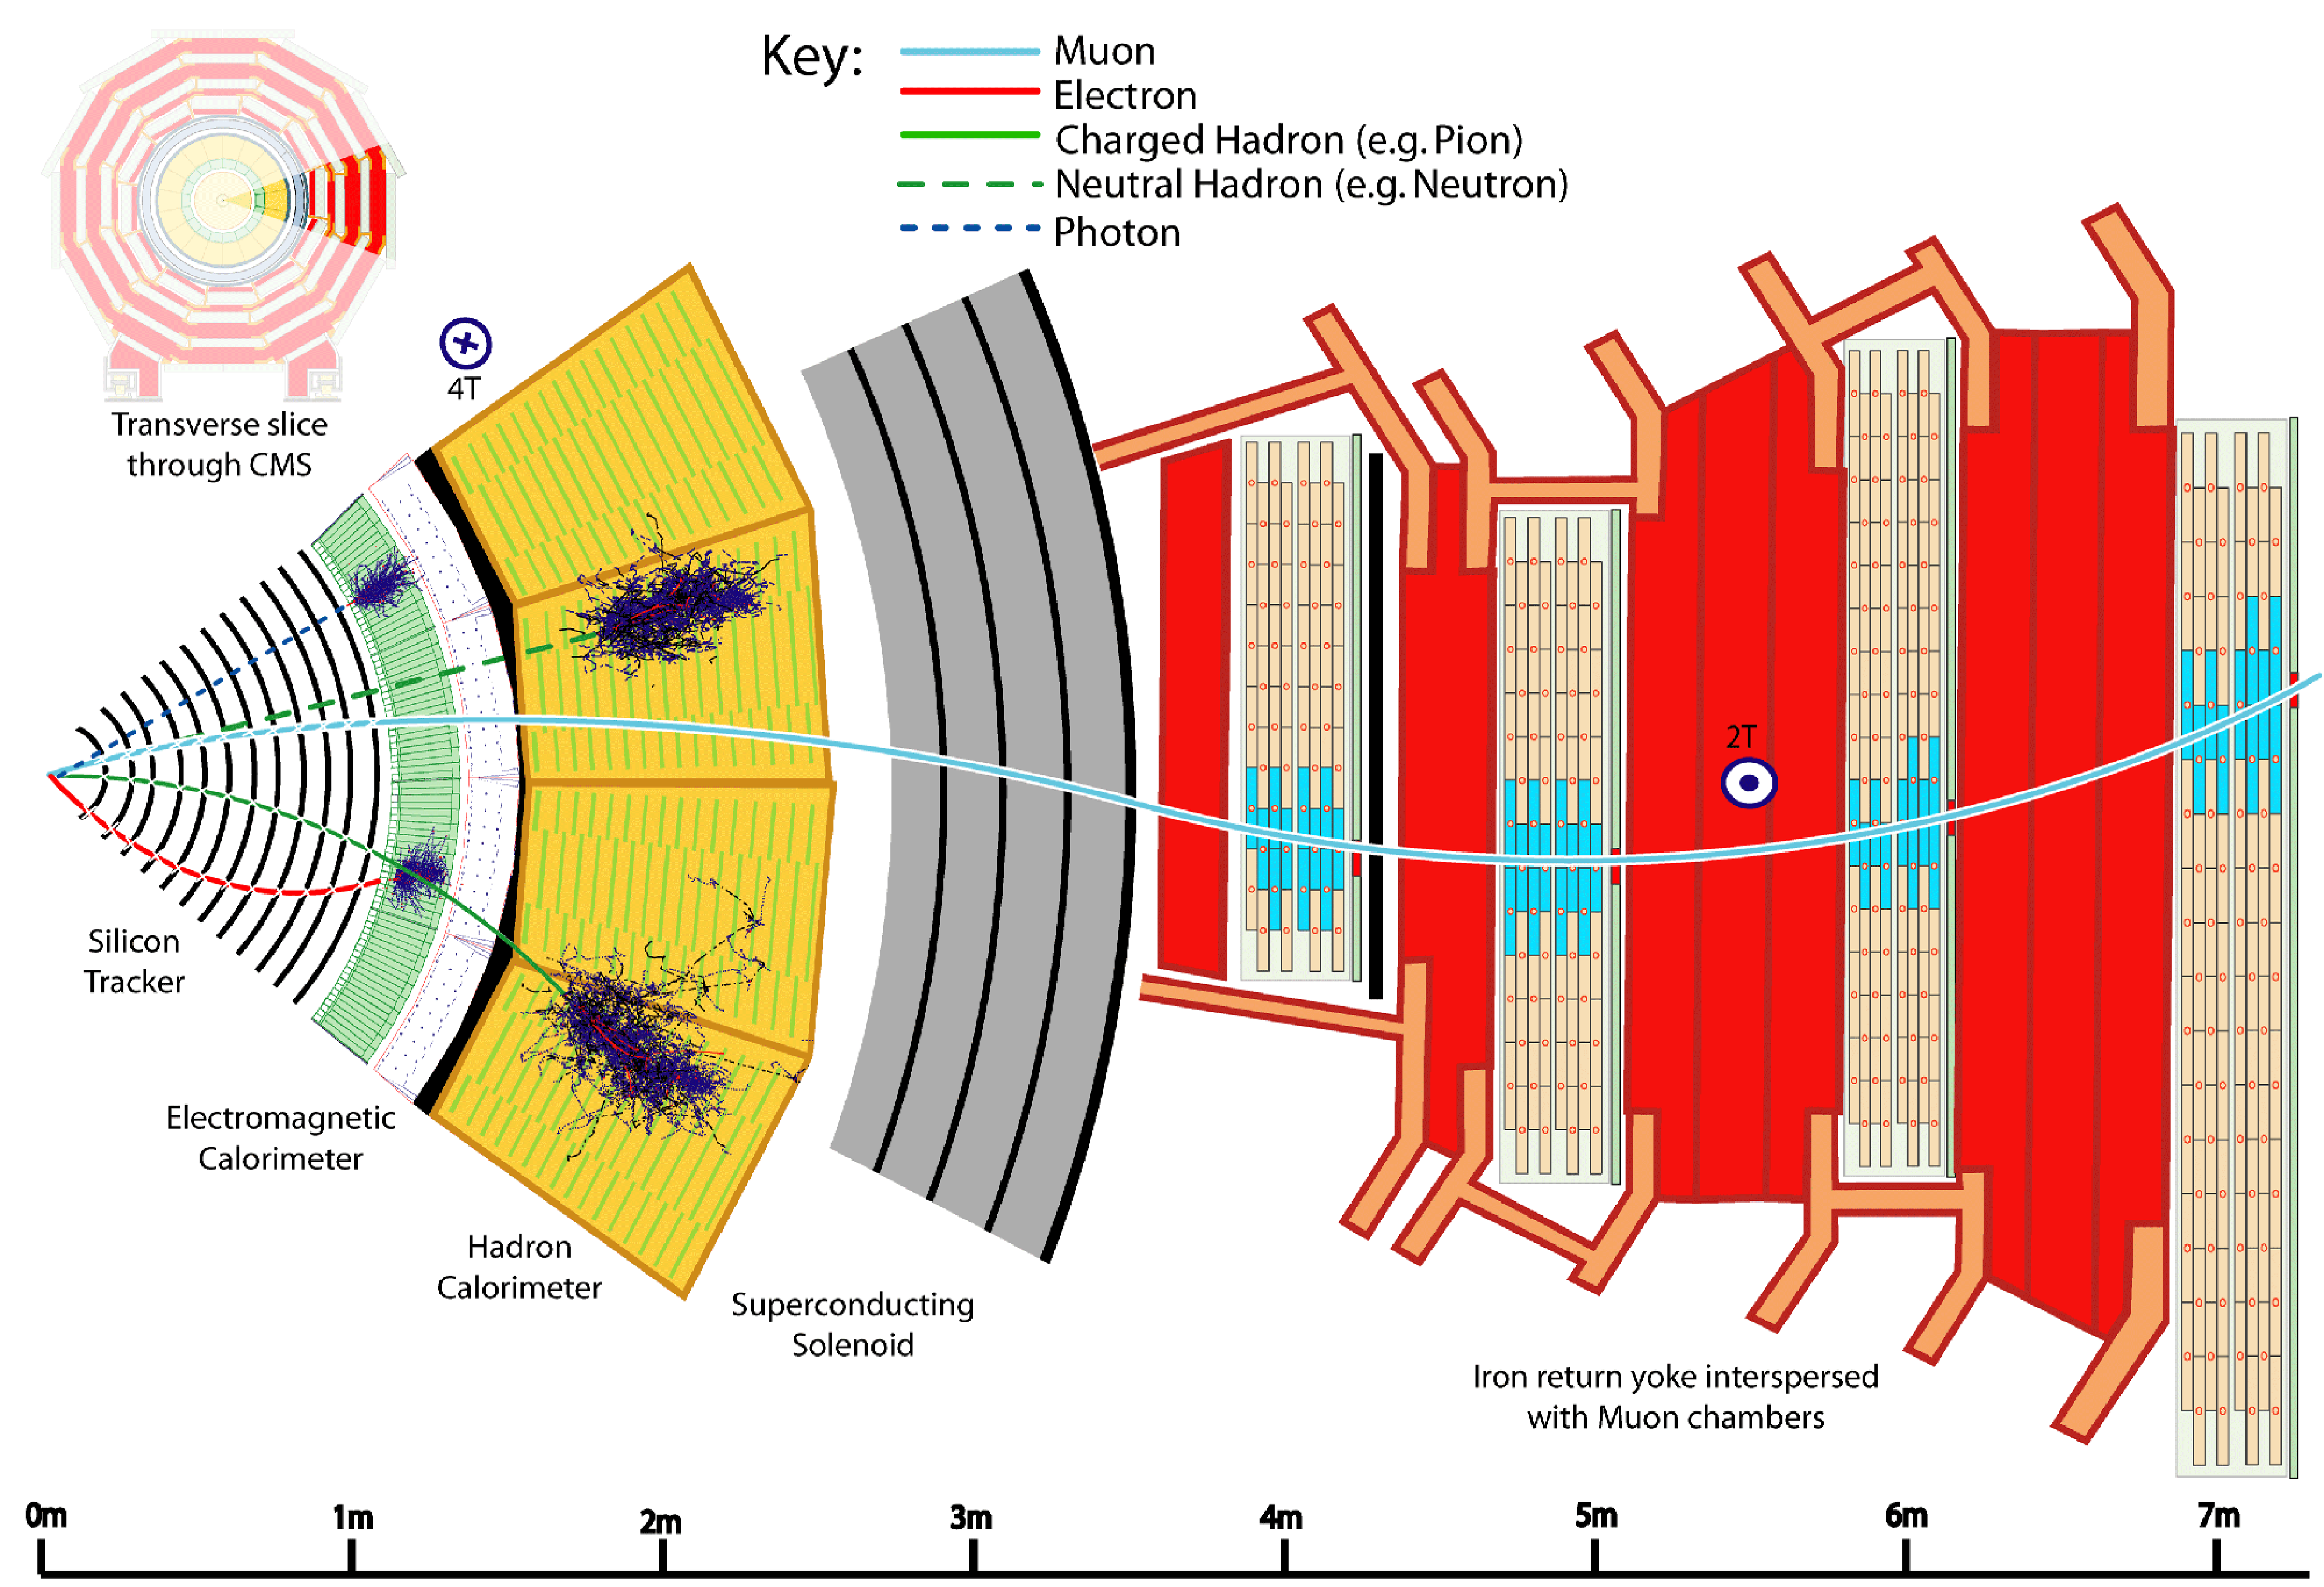
\includegraphics[width=\hugefigwidth]{chap_CMSDetector_figures/cms_slice}
  \caption[CMS Detector Slice figure]%
  {CMS detector figure slice}
  \label{fig:CMSFigureSlice}
\end{figure}

The coordinate system of CMS has its origin inside the detector at the primary
interaction point. The x-axis points radially towards the center of the
LHC, whereas the y-axis points vertically upward. Thus, the z-axis shares the
same direction with the beam line. The azimuthal angle $\phi$ is measured from
the x-axis in the x-y plane whereas the polar angle $\theta$ is measured from the z-axis.

Particle physicists often use a quantity called rapidity
$y$ instead of $\theta$. It is defined as:

\begin{equation}
\label{eq:CMSqd1}
 y = \frac{1}{2} \,\ln \frac{E + p_z}{E - p_z} \, = tanh^{-1} \,\frac{p_z}{E}
\end{equation}

and equals, in case of massless particles, the pseudorapidity $\eta $ given by

\begin{equation}
\label{eq:CMSqd2}
 \eta = -\ln[\tan(\theta/2)]
\end{equation}

The use of rapidity instead of the polar angle is motivated by the fact that the difference 
in rapidity between two particles is invariant under Lorentz boosts along the beam axis

The angular distance between two particles observed from the origin of the
coordinate system is

\begin{equation}
\label{eq:CMSqd3}
\Delta R = \sqrt{\Delta \phi^2 + \Delta \eta^2} 
\end{equation}

Measurable quantities like momentum and energy transverse to the beam line
are denoted by $p_T$ and $E_T$ , respectively, and can be derived from its x and
y components. The CMS detector is located north of the LHC center. The
origin of the CMS coordinate system is the CMS collision point. Neglecting
the small tilt of the LEP/LHC plane.

\subsection{Magnet}

The superconducting solenoid magnet reaches a maximum magnetic field of 3.8 
T in the positive z direction in the inner detectors. A high magnetic field provides 
a large bending power in the transverse plane for charged particles, which makes 
possible to reach precise measurement of muon momenta. The magnet is 12.5 m long 
and with an inner radius of 6 m and is made of four-layers of NbTi. It is the largest 
superconducting magnet ever built, with the capacity to store an energy of 2.6 GJ at 
full current. The magnetic flux is returned via a 1.5 m thick iron yoke instrumented 
with four stations of muon chambers. In this part of the detector the magnetic field 
is saturated at 2 T. More detailed information can be found in reference \cite{CMSMagnet} 
Figure \ref{fig:CMSMagnet} shows artistic view of CMS magnet, a huminoid is also persent
on figure to highlight the huge size of magnet.
\begin{figure}
  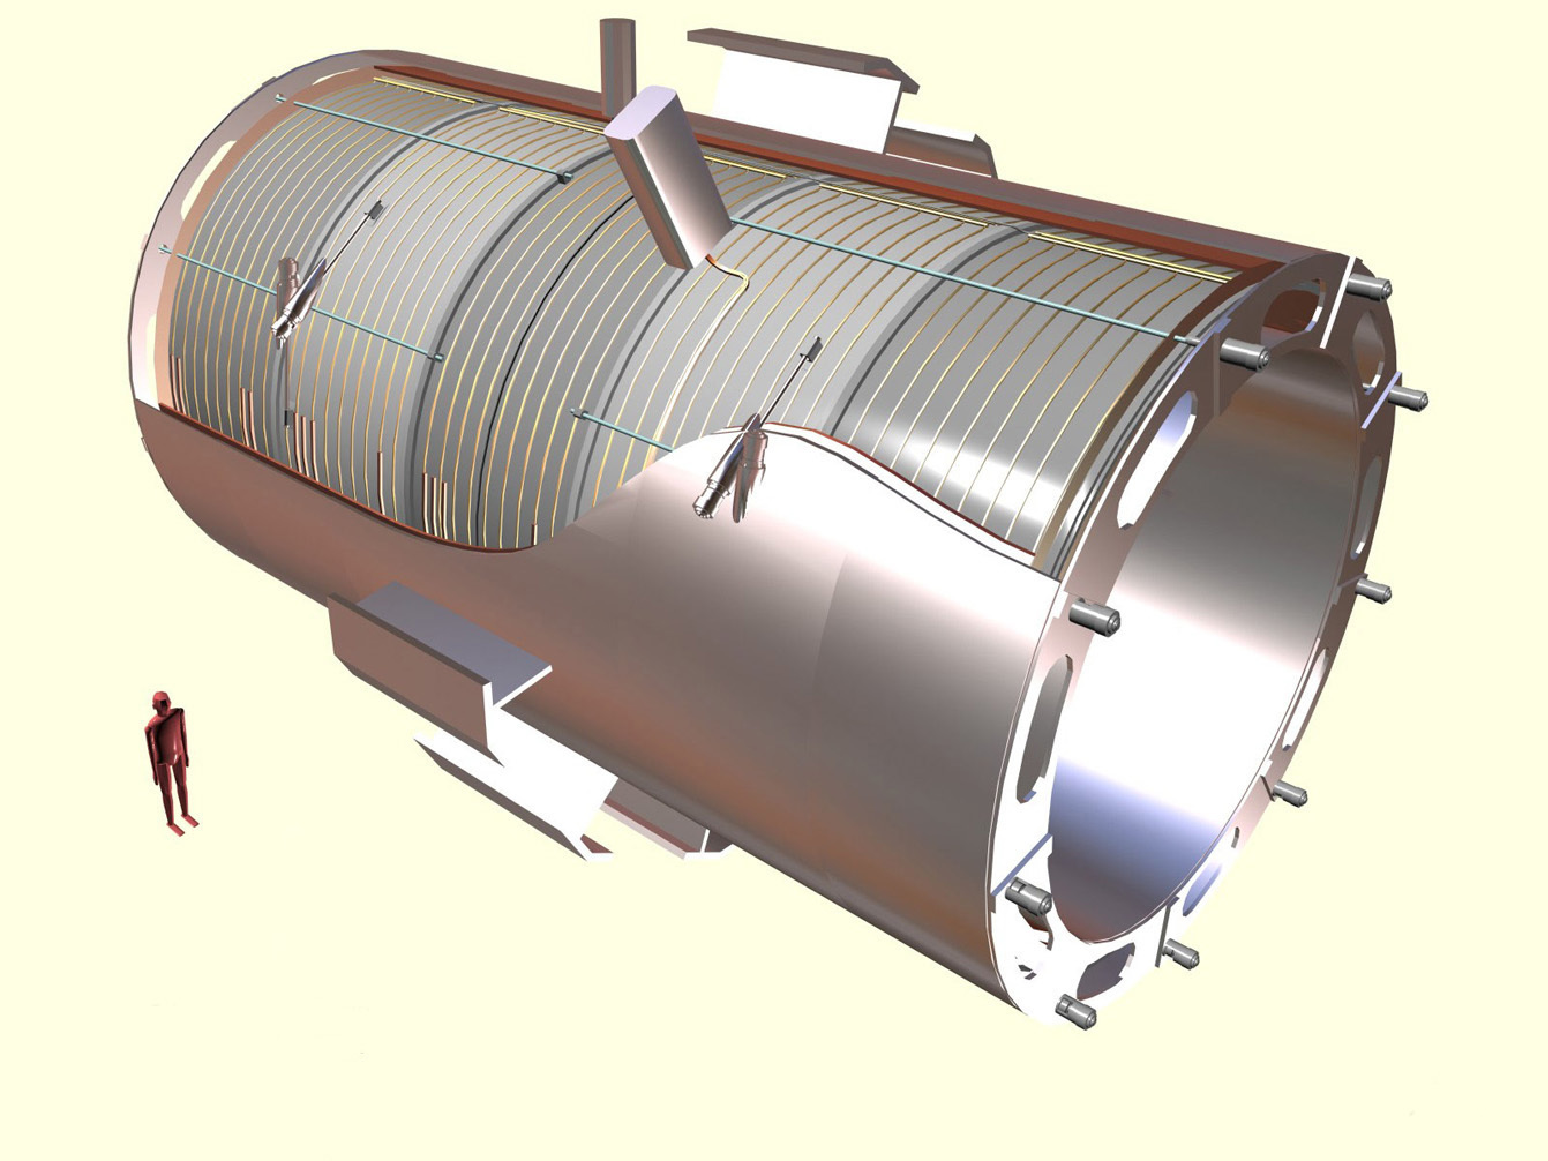
\includegraphics[width=\largefigwidth]{chap_CMSDetector_figures/cms_magnet}
  \caption[CMS Magnet artistic view]%
  {CMS Magnet }
  \label{fig:CMSMagnet}
\end{figure}



\subsection{Tracker}

The Tracker is the subdetector system which is closest to the interaction point, 
a general layout is presented in Figure \ref{fig:CMSTracker} It is designed to provide an efficient mea- 
surement of the trajectories of charged particles emerging from the LHC collisions, as 
well as a precise reconstruction of secondary vertices. The CMS Tracking System is 
composed of q silicon pixel detector close to the interaction region and a strip detector 
covering radii from 0.2 m to 1.1 m. The Pixel Detector consists of 1440 pixel modules 
arranged in three barrel layers and two disks in each end-cap. The barrel layers are 
located at radii of 4.4, 7.3 and 10.2 cm around the interaction point with a length of 
53 cm. On each side of the barrel, two discs are placed at $|z|$ = 32.5 cm and 46.5 cm.

\begin{figure}
  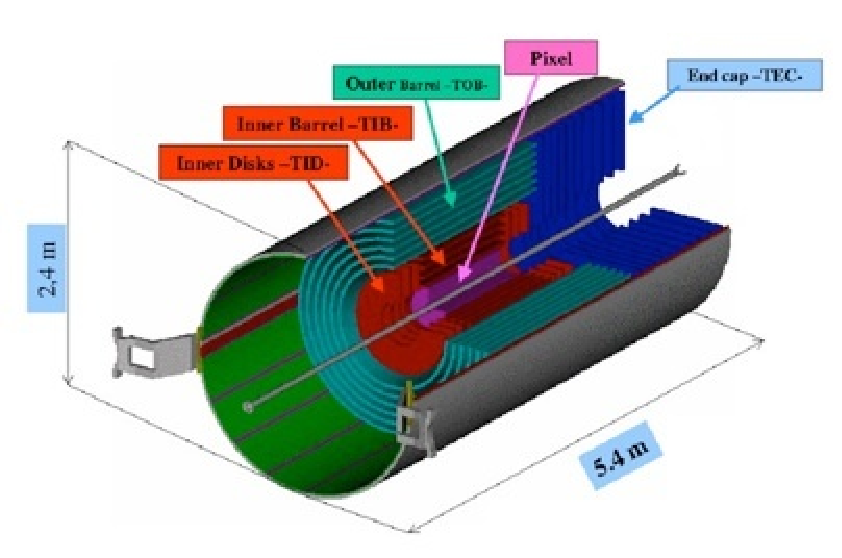
\includegraphics[width=\largefigwidth]{chap_CMSDetector_figures/cms_tracker_3d_drawing}
  \caption[CMS Tracker 3D drawing]%
  {CMS Tracker drawing}
  \label{fig:CMSTracker}
\end{figure}


\subsection{Calorimetry}

{\bf ECAL} \\


The electromagnetic calorimeter (ECAL) is used to measure the energy of photons 
and electrons. The ECAL is a high precision scintillating crystal calorimeter. The 
structure of the ECAL can be seen in Figure \ref{fig:CMSECAL}. It is composed of 61,200 lead tungstate 
(PbWO$_4$) crystals in the barrel region and 7,324 crystals in the endcaps. The choice 
of that material is motivated by its fast response and high radiation resistance and 
its very good resolution. In front of each ECAL Endcap is a preshower detector (ES),
from 1.65 $ \leq |\eta| \leq$ 2.6 made from silicon strip detectors in order to identify neutral 
pions ($\pi^0$). The nominal energy resolution, measured with electron beams having 
momenta between 20 and 250 GeV, is:
 
\begin{equation}
\label{eq:eqnECAL}
%\Delta R = \sqrt{\Delta \phi^2 + \Delta \eta^2} 
\frac{\sigma_E}{E}=(\frac{S}{\sqrt{E}})^2 + (\frac{N}{E})^2 + C^2.
\end{equation}


where S is the stochastic term, which includes fluctuations in the shower containment 
as well as a contribution from photostatistics, N is the noise term, which accounts 
for the electronic, digitization, and pileup noise, and C is the constant term, which 
comes from the light collection non-uniformity, errors on the inter-calibration among 
the modules, and the energy leakage from the back of the crystal.\\

\begin{figure}
  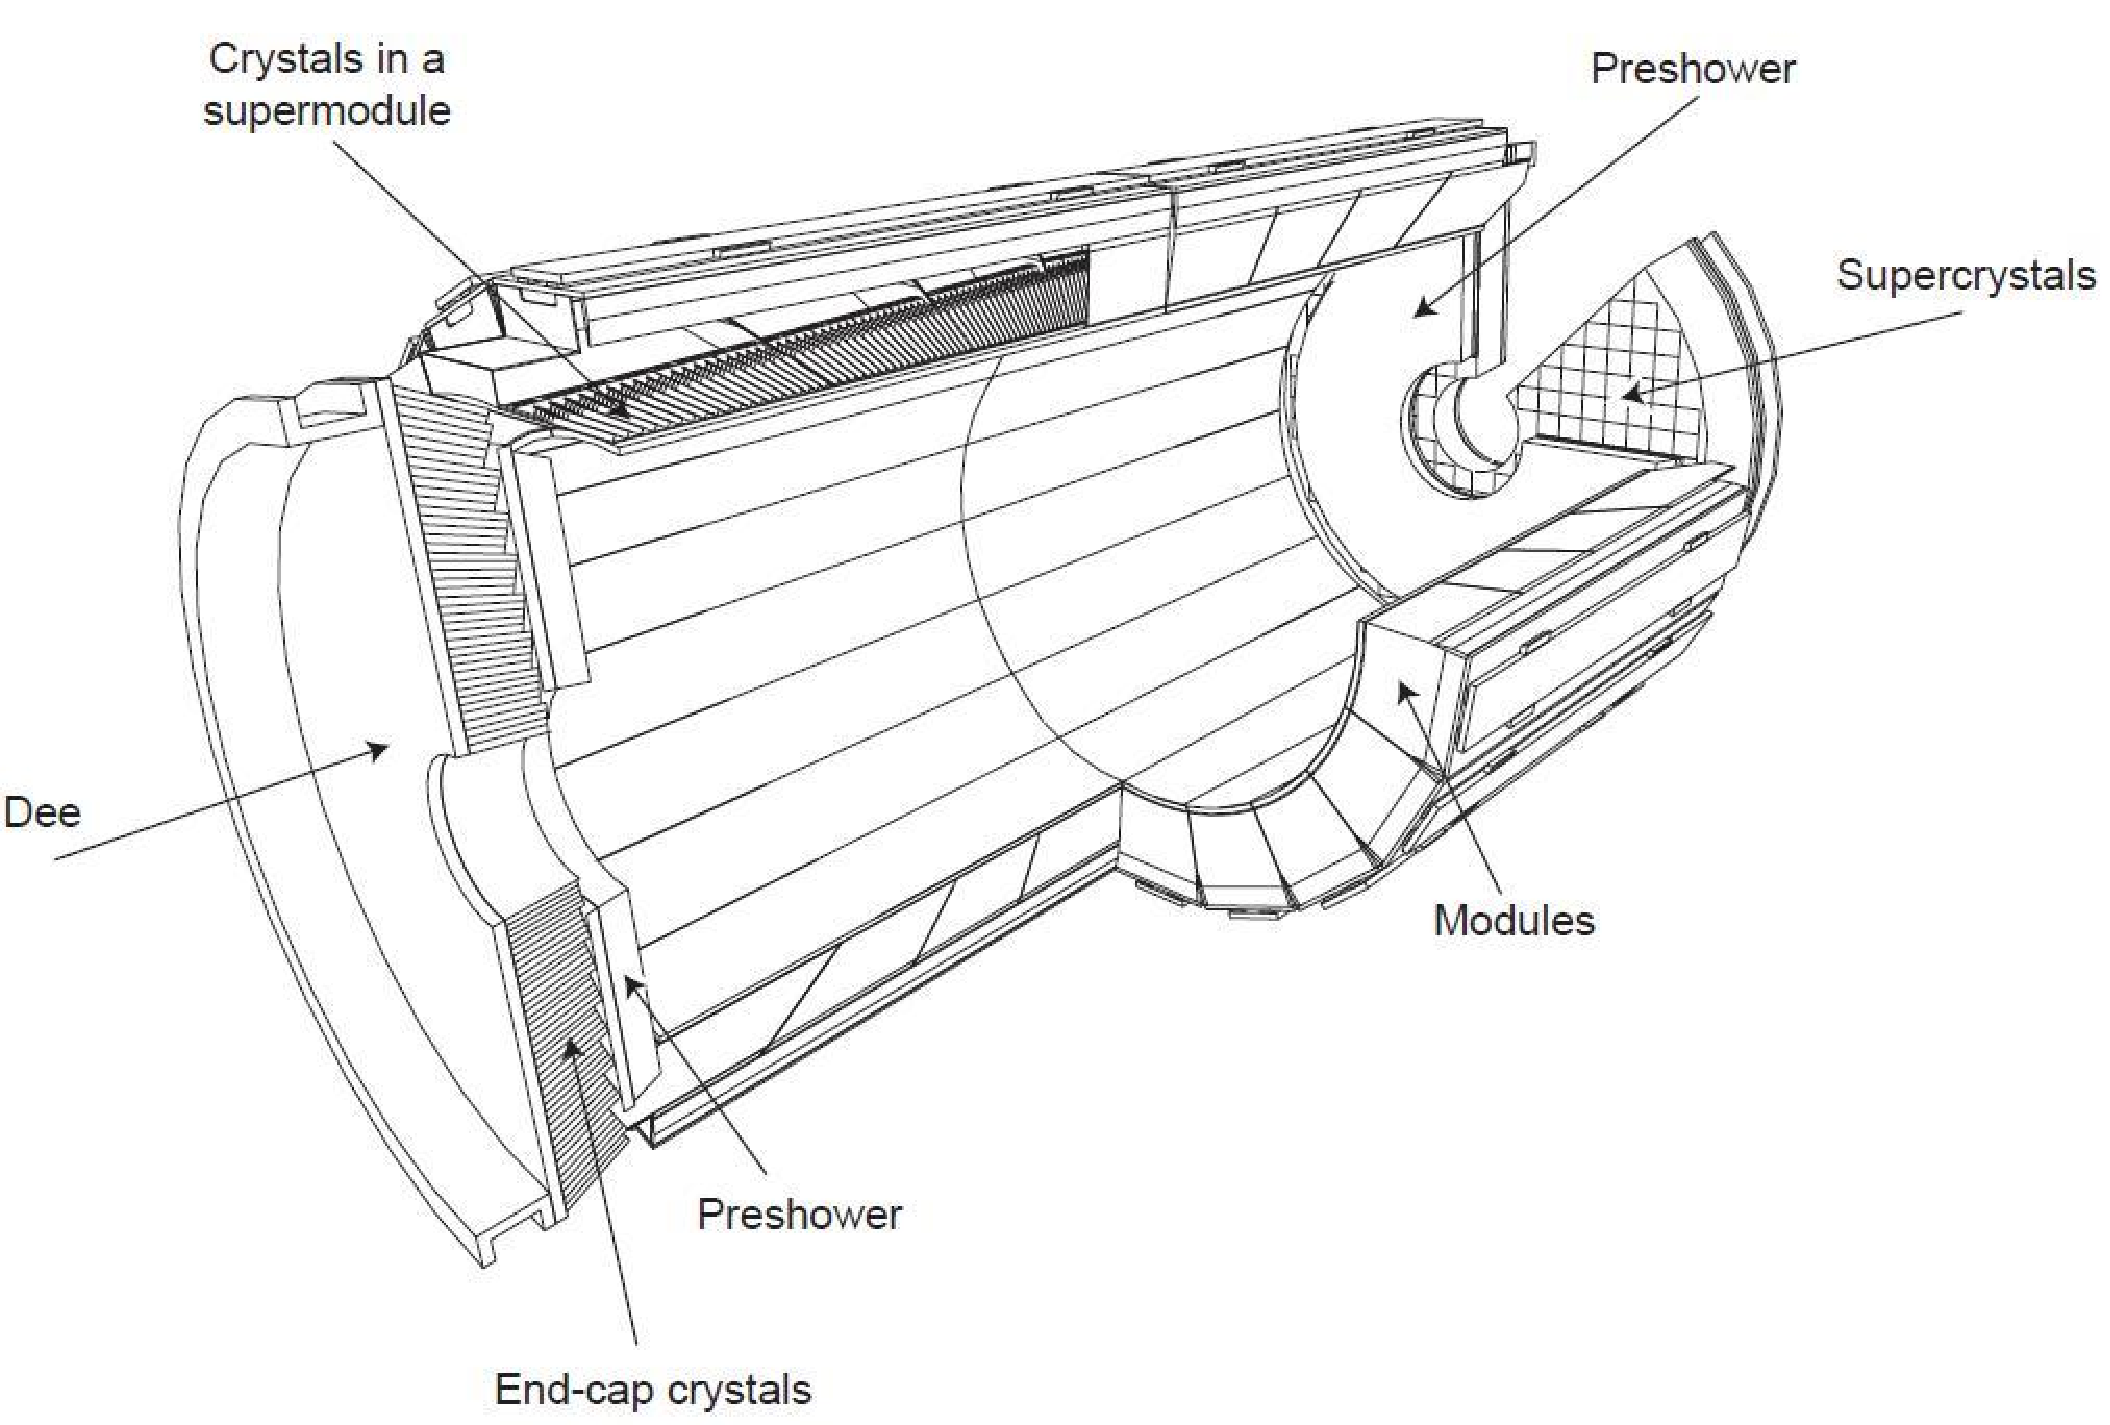
\includegraphics[width=\largefigwidth]{chap_CMSDetector_figures/cms_ECAL}
  \caption[CMS ECAL]%
  {CMS ECAL detector}
  \label{fig:CMSECAL}
\end{figure}


{\bf HCAL}  \\

The hadronic calorimeter (HCAL) is designed to measure the energy of hadrons. 
The HCAL is comprised of four subsystems: the HCAL Barrel (HB), the outer 
calorimeter (HO), the HCAL Endcap (HE), and the forward calorimeter (HF). 
Figure \ref{fig:CMSHCAL} gives a schematic overview on the HCAL sub-detector. 
The HB is a sampling calorimeter that covers the range $|\eta| < $ 1.3. 
It consists of 36 identical azimuthal wedges aligned parallel to the beamline. 
It is located between the ECAL and the 
solenoid coil and is supplemented by the HO located between the solenoid and the 
muon chambers. The HO is designed to absorb the remnant of the hadronic shower 
which has not been fully absorbed in the HB. The HE covers a large portion of the 
solid angle, 1.3 $< |\eta| < 3$. Beyond that region, the HF placed at 11.2 m from the 
interaction point extends the pseudorapidity coverage up to $|\eta|$ < 5.2. The HE must 
have high radiation tolerance, with 10 Mrad expected after 10 years of operation. 
The reason for the absorber material to be non-magnetic is that it must not affect 
the magnetic field. The HF experiences the harshest radiation environment and therefore 
requires an extremely radiation tolerant material. The active material chosen is 
quartz fibers.
The fibers are mounted in grooves in the steel absorber plates. The inner part of the HF will be 
exposed to close to 100 Mrad/year. As the absorber will become radioactive the entire HF can be moved into
a garage to limit exposure of personnel during maintenance periods.


\begin{figure}
  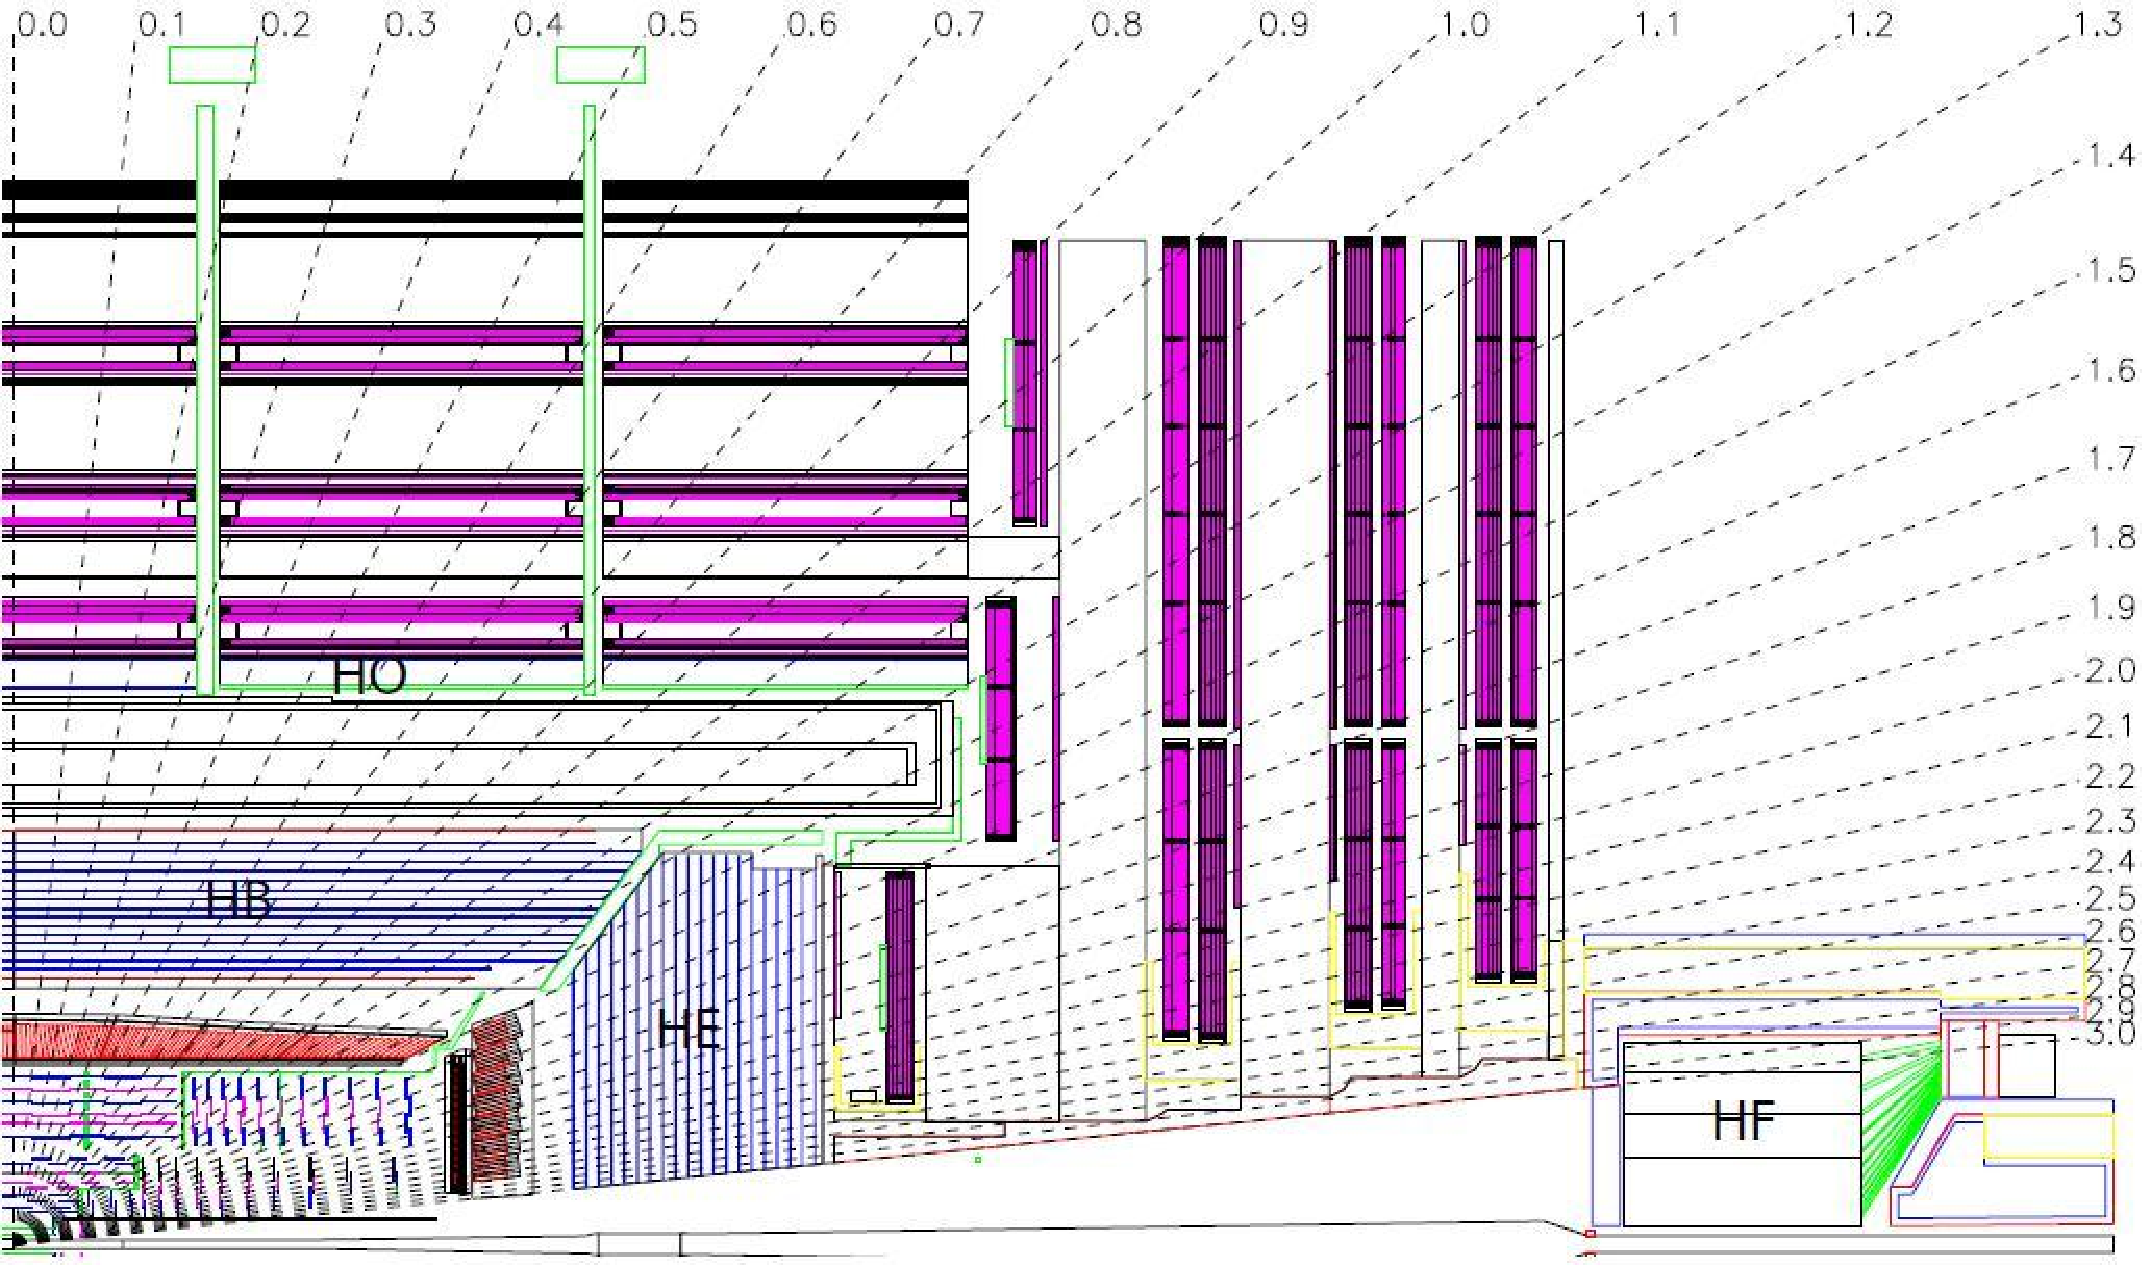
\includegraphics[width=\largefigwidth]{chap_CMSDetector_figures/cms_HCAL}
  \caption[CMS HCAL]%
  {CMS HCAL detector}
  \label{fig:CMSHCAL}
\end{figure}


\subsection{CMS Muon System}

One of the main design objectives of the CMS detector was to obtain a high precision
muon momentum measurement, for its key role both in new physics searches and
in Standard Model measurements. The CMS muon system \cite{CMSExp} uses three diffrent
types of gaseous detectors to detect muons. In the barrel region, Drift Tubes (DTs)
and Resistive Plate Chambers (RPCs) are used, while in the endcap there are Cathode
Strip Chambers (CSCs) and also RPCs. The layout of the CMS muon system is shown in 
Figure \ref{fig:CMSMuonSystem}. \\



\begin{figure}
  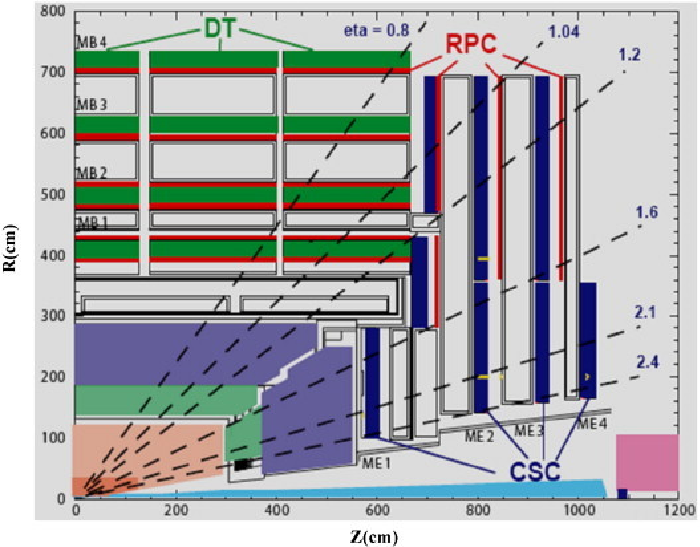
\includegraphics[width=\largefigwidth]{chap_CMSDetector_figures/CMSMuonSystem}
  \caption[CMS Muon system]%
  {CMS Muon system}
  \label{fig:CMSMuonSystem}
\end{figure}


{\bf Drift Tubes} \\

In the central region of CMS, $|\eta| <$ 1.2, the muon system consists of four concentric
cylinders containing 250 gas drift chambers. Each Drift Tube is filled will a mix of
85$\%$ Argon and 15$\%$ CO$_2$ with active wires for charge collection. As muons pass
through the gas they leave an ionization trail. The charge drifts to the wires, which
detect the charge. The size of the drift cell was chosen so the maximum drift time is
380 ns. There are $~$172000 active wires in the entire system. The use of DTs is only
possible in this region due its low magnetic field.\\


{\bf Cathode Strip Chambers} \\

In the endcap, the muon system is comprised of Cathode Strip Chambers (CSC).
The CSC's cover the 0.9$<|\eta|<$2.4 pseudorapidity range. Each CSC is trapezoidal
in shape and consists of 6 gas gaps, each gap having a plane of radial cathode strips
and a plane of anode wires running almost perpendicularly to the strips. The CSC is
a fast detector (response time of $~$4.5 ns), but with rather coarse position resolution;
a precise position measurement is made by determining the centre-of-gravity of the
charge distribution induced on the cathode strips (spatial resolution $~$200 $\mu$m, angular
resolution $~$10 mrad).\\


{\bf Resistive Plate Chambers} \\

In order to improve muon trigger system and for a good measurement of the bunch
crossing time, resistive plate chambers (RPC) are mounted in the barrel and endcap
region ($|\eta| < $1.6). The RPCs are able to provide independent and fast trigger with
high segmentation and sharp pT threshold over a large portion of the pseudorapidity
range. However, the RPCs have coarser position resolution making them more useful
for the trigger

\subsection{Trigger and Data Acquisition}

The CMS trigger system is designed to cope with an unprecedented high luminosity
and interactions rates. The LHC will collide proton bunches at a rate of 40
MHz which leads to $~$10$^9$ interactions per second at design luminosity. Since it is
not possible to record events at this rate, a two-part trigger system, consisting of a
hardware-based trigger (Level 1) and a software-based trigger (High Level Trigger) is
used \cite{CMSTrigger1,CMSTrigger2}. The rate is then reduced by a factor of 10$^6$.\\


{\bf Level 1 Trigger} \\
The Level 1 (L1) trigger is designed to achieve a maximum output rate of 100
kHz and consists of custom-designed, programmable electronics. The front-end (FE)
electronics can store information from up to 128 consecutive events, which equates
to $~$3 $\mu$s. To cope with the time limitation, the L1 trigger system uses only coarsely
segmented data from the muon system and the calorimeters while the full granularity
data are stored in the FE electronics waiting for the L1 decision. The L1 muon trigger
is organized into subsystems representing the three different muon detectors: the DT
trigger in the barrel, the CSC trigger in the endcap and the RPC trigger covering
both barrel and endcap. The Level-1 muon trigger also has the Global Muon Trigger
(GMT) that combines the trigger information from the DT, CSC, and RPC muon
subsystems, as well as from the calorimeter subsystem, and sends it to the Level-1
Global Trigger.\\


{\bf High Level Trigger }\\

The High Level Trigger (HLT) exploits the full amount of collected data for each
bunch crossing accepted by Level 1 Trigger and is capable of complex calculations
such as the offine ones. It is structured in two levels, Level 2 (L2) and Level 3
(L3) implemented in software. The L2 uses information from the muon spectrometer
(parameters from the L1 muon candidates converted into seeds) to perform a standalone
reconstruction, providing a muon pT measurement with a precision of about
15 $\%$. The L2 reconstruction follows closely the offine standalone reconstruction using
Kalman-filter techniques. The L3 takes L2 candidates as seeds and adds information
from the inner tracker by performing track reconstruction in the silicon tracker. This
reconstruction is regional, it performs pattern recognition and track fitting only in
a small $\eta - \phi $ slice of the tracker, to keep execution time low. Trajectories are then
reconstructed using Kalman-filter techniques. Level 3 provides a much more precise
p$_T$ measurement (1$\%$ - 2$\%$ in the barrel region) than Level 2, as well as the ability
to select on the basis of the track impact parameter with respect to the beam spot.
After the HLT decisions, the event rate decreases down to 100Hz for mass storage
which corresponds to a data rate of 150 Mbyte$/$s.


\subsection{CMS data flow}
Raw data that passed HLT and CMS Online Data Acquisition system (system which collects
data from different detectors and builds events) is stored at a storage facility at CERN, known
as Tier-0. The raw data contains information for every single proton-proton collision which
passed HLT and it is called an event. There are about 10$^9$ events per year stored at Tier-0.
Standard CMS algorithms perform calibration and alignment of the detector using raw data
and do prompt (first) reconstruction of physics objects like muons, electrons, jets etc. Later,
their momenta, energies and trajectories are measured and this is done by using all detectors
of CMS experiment.
The output data from prompt reconstruction is saved in different primary datasets based on
trigger information.
The data from Tier-0 is transferred to Tier-1 storage facilities worldwide where further calibration
and re-reconstruction is performed centrally to be used by all CMS analyzes. The
Tier-2 centers are more numerous and they are based at different universities in the world.
They have limited disk space and are used for running individual analysis and Monte Carlo
simulations.
Data is stored in three types of root files which contain information about raw, reconstructed
and analysis object data, respectively RAW, RECO and AOD root files. The RAW root files
contain information about the recorded event in raw format as hits, energy deposits in the detector
etc. The RECO root files contain detailed information of reconstructed physics objects
and the AOD root files are simplified version of the RECO files which are mostly used in the
analyses.
Tier-0, Tier-1 and Tier-2 centers form a GRID \cite{LHCGrid} based computer infrastructure in 35 countries.

